\chapter{Simulations}\label{chapter:simulations}
\section{Biot Savart field simulations}
	\subsection{$B_0$ fields in low field NMR}
		For $B_0$ field generation, mostly solenoid coils with compensation windings on both ends
		were used. To find optimal lengths and numbers of layers, Matlab simulations of static fields using Biot Savart's law were implemented.
		Both solenoidal structures and "closed" loops were simulated.
		The measure considered was absolute field distribution inside a volume of
		$\SI{3}{\centi\meter}$ by  $\SI{3}{\centi\meter}$ by $\SI{3}{\centi\meter}$. 
		fields were calculated in a grid of \todo{30 cubed} points. Absolute field difference inside the volume was considered first and then refined by
		histogram evaluation which yields results similar to the lorentian distribution a fourier transformed NMR signal shows. To estimate linewidths generated by field inhomogenyeties, the conservative measure of the central 80 \% of field points was used.
		Using this representation and varying different parameters such as diameter, distances and relative currents in different loop structures, optimal geometries for different coil designs were calculated.
		\subsection{Solenoid Coil}
			The field of an infinitely long solenoid would be almost perfectly homogeneous along its symmetry axis. Due to the limited
		\subsection{Additional Compensation Windings}
			Additional compensation windings further smoothed the field by adding a differently shaped field component that can be used to partly compensate the solenoids inhomogenieties. Figure \todo{nn} shows the fields of solenoid and and compensation windings in the x-z-plane and the resulting superposition.
			To evaluate the field in the 3D sample volume, histograms of the field distribution were generated for different compensation wind lenghts. As visible in figure nn, the influence of a single wind are quite substantial indicating that the manufacturing process must be well controlled. Additionally, it can be seen that
			\begin{figure}[b]
				\centering
				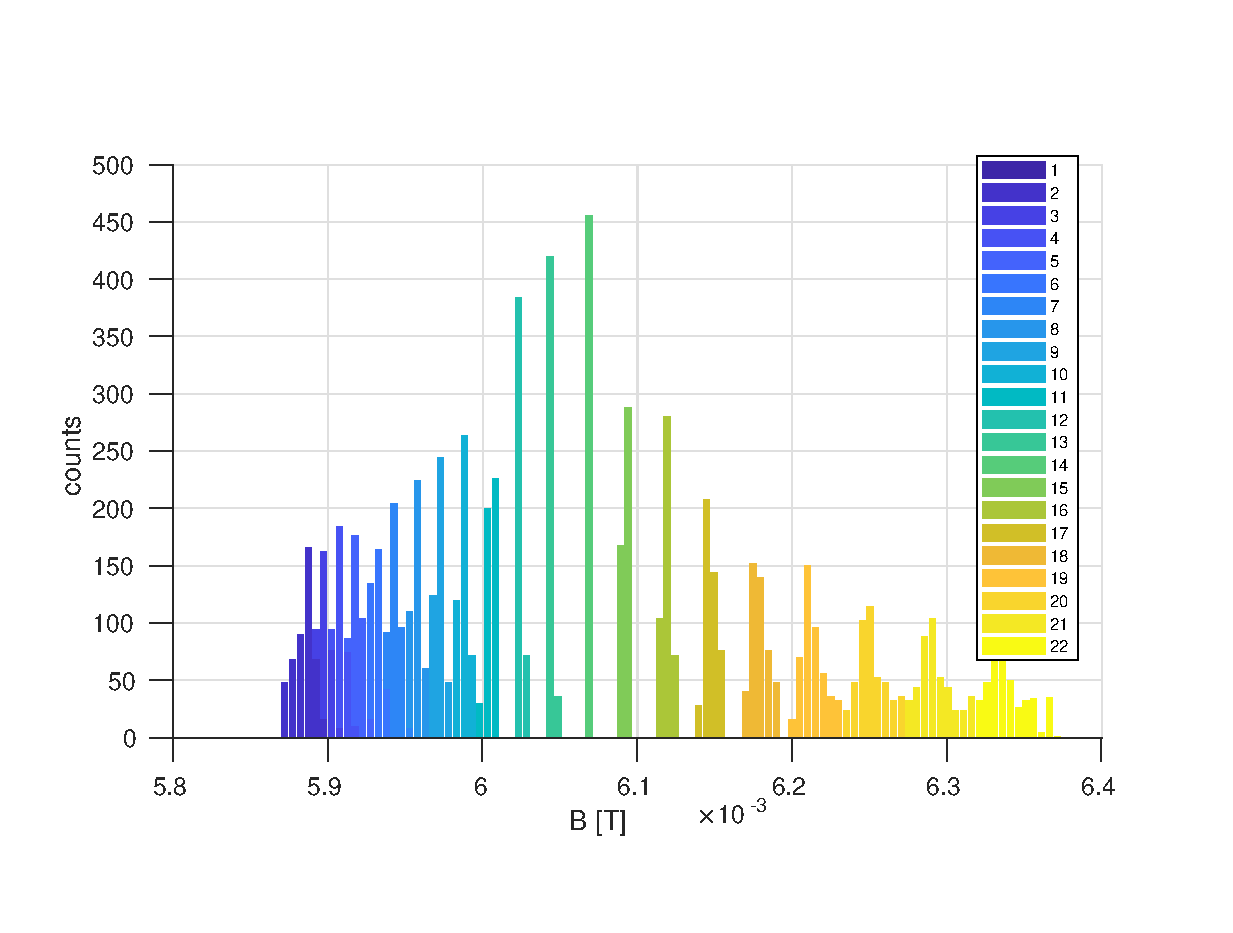
\includegraphics[width=\textwidth]{/home/philipp/Documents/thesis/figures/simulations/compensationWinds.eps}
				\caption{Histograms of the magnetic field strength. From left to right, number of compensation windings rise. This leads to a field increase and change in homogeniety.}
			\end{figure}

		\subsection{Dual Helmholtz Array}
			As a more advanced setup that is less prone to manufacturing errors due to the relatively larger distances to the sample volume, a dual helmholtz array design was considered. A single Helmholtz array provides less Homogeniety than a solenoid (Fig ..) but the additional pair of coils generates a differently shaped field similar to the compensation windings for the solenoid. By variation of the distances of both pairs relative to the center and their respective field strengths, i.e. the currents of the coil pairs, optimal parameters were extracted from the simulations. The 
	\section{Simulations using the groups' spin dynamics\todo{name?} framework}
		To estimate the 
